%%%%%%%%%%%%%%%%%%%%%%%%%%%%%%%%%%%%%%%%%
% Short Three-Column Newsletter
% LaTeX Template
% Version 1.0 (11/9/13)
%
% Original author:
% Frits Wenneker (http://www.howtotex.com) 
% With extensive modifications by:
% Vel (vel@latextemplates.com)
% 
% This template has been downloaded from:
% http://www.LaTeXTemplates.com
%
% License:
% CC BY-NC-SA 3.0 (http://creativecommons.org/licenses/by-nc-sa/3.0/)
%
%%%%%%%%%%%%%%%%%%%%%%%%%%%%%%%%%%%%%%%%%

%----------------------------------------------------------------------------------------
%	PACKAGES AND DOCUMENT CONFIGURATIONS
%----------------------------------------------------------------------------------------

\documentclass[10pt,a4paper]{article} % Paper type (a4paper, usletter or legal) and font size (10, 11 or 12)

\setlength\topmargin{-48pt} % Top margin
\setlength\headheight{0pt} % Header height
\setlength\textwidth{7.0in} % Text width
\setlength\textheight{9.5in} % Text height
\setlength\oddsidemargin{-30pt} % Left margin
\setlength\evensidemargin{-30pt} % Left margin (even pages) - only relevant with 'twoside' article option

\usepackage{charter} % Charter font for main content
\usepackage{siunitx}
\frenchspacing % Reduces space after periods to make text more compact for a three-column layout

\usepackage{graphicx} % Required for including images
\usepackage{amssymb,amsmath} % Math packages
\usepackage{multicol} % Required for the three-column layout of the document
\usepackage{url} % Clickable links
\usepackage{enumitem} % Reduces the amount of space within and between lists with [noitemsep,nolistsep]
\usepackage{marvosym} % Required for the use of symbols
\usepackage{wrapfig} % Allows wrapping text around figures
\usepackage[T1]{fontenc} % Use 8-bit encoding that has 256 glyphs
\usepackage{datetime} % Required for defining a custom date style
\newdateformat{mydate}{\monthname[\THEMONTH] \THEYEAR} % Set a custom date format
\usepackage[pdfpagemode=FullScreen, colorlinks=false]{hyperref} % Link colors and PDF behavior in Acrobat
\usepackage{fancyhdr} % Required to define custom headers/footers
\pagestyle{fancy} % Enables the custom headers/footers for all pages following this

%-----------------------------------------------------------
% Header and footer
\lfoot{\footnotesize % Left footer containing newsletter contact information
	Studying in four different countries during my Master Degree\\
	\Mundus\ \href{https://github.com/stefanos1316/my_blog/index.com}{my\_blog/index.com} \quad
	%\Telefon\ Not available yet \quad
	\Letter\ \href{mailto:sgeorgiou@aueb.gr}{sgeorgiou@aueb.gr}
}


\cfoot{} % Empty center footer

\rfoot{\footnotesize ~\\ Page \thepage} % Right footer - page counter

\renewcommand{\headrulewidth}{0.0pt} % No horizontal rule for the header
\renewcommand{\footrulewidth}{0.4pt} % Horizontal rule separating the footer from the document
%-----------------------------------------------------------

%-----------------------------------------------------------
% Define separators
\newcommand{\HorRule}[1]{\noindent\rule{\linewidth}{#1}} % Creates a horizontal rule
\newcommand{\SepRule}{\noindent	% Creates a shorter separator rule
\begin{center}
\rule{250pt}{1pt} % Page width and rule width
\end{center}
}
%-----------------------------------------------------------

%-----------------------------------------------------------
% Define title and article styles
\newcommand{\NewsletterName}[1]{ % Newsletter title
\begin{center}
\Huge \usefont{T1}{fvs}{b}{n} % Use the Bera Sans Bold font
#1
\end{center}	
\par \normalsize \normalfont}

\newcommand{\JournalIssue}[1]{ % Date and issue number at the top of the newsletter
\hfill \textsc{\mydate \today, No #1} % Right-aligned date and issue number
\par \normalsize \normalfont}

\newcommand{\NewsItem}[1]{ % News item title
\usefont{T1}{fvs}{n}{n} % Use the Bera Sans Normal font
\vspace{24pt}\large #1\vspace{3pt} % Print the title with space around it in a larger font size
\par \normalsize \normalfont}

\newcommand{\NewsAuthor}[1]{ % Author name under the item title
\hfill by \textsc{#1} \vspace{20pt} % Right-aligned author name in small caps with space after it
\par \normalfont}		

%----------------------------------------------------------------------------------------
%	TITLE
%----------------------------------------------------------------------------------------

\begin{document}

\JournalIssue{1} % Issue number

\NewsletterName{Studying in four different countries} % Newsletter title

\noindent\HorRule{3pt} \\[-0.75\baselineskip] % Thick horizontal rule
\HorRule{1pt} % Thin horizontal rule

%----------------------------------------------------------------------------------------
%	MAIN NEWS ITEM
%----------------------------------------------------------------------------------------

\vspace{0.5cm}
\SepRule
\vspace{-0.5cm}

\begin{center}
\begin{minipage}[h]{0.75\linewidth}
\begin{wrapfigure}{l}{0.45\textwidth}
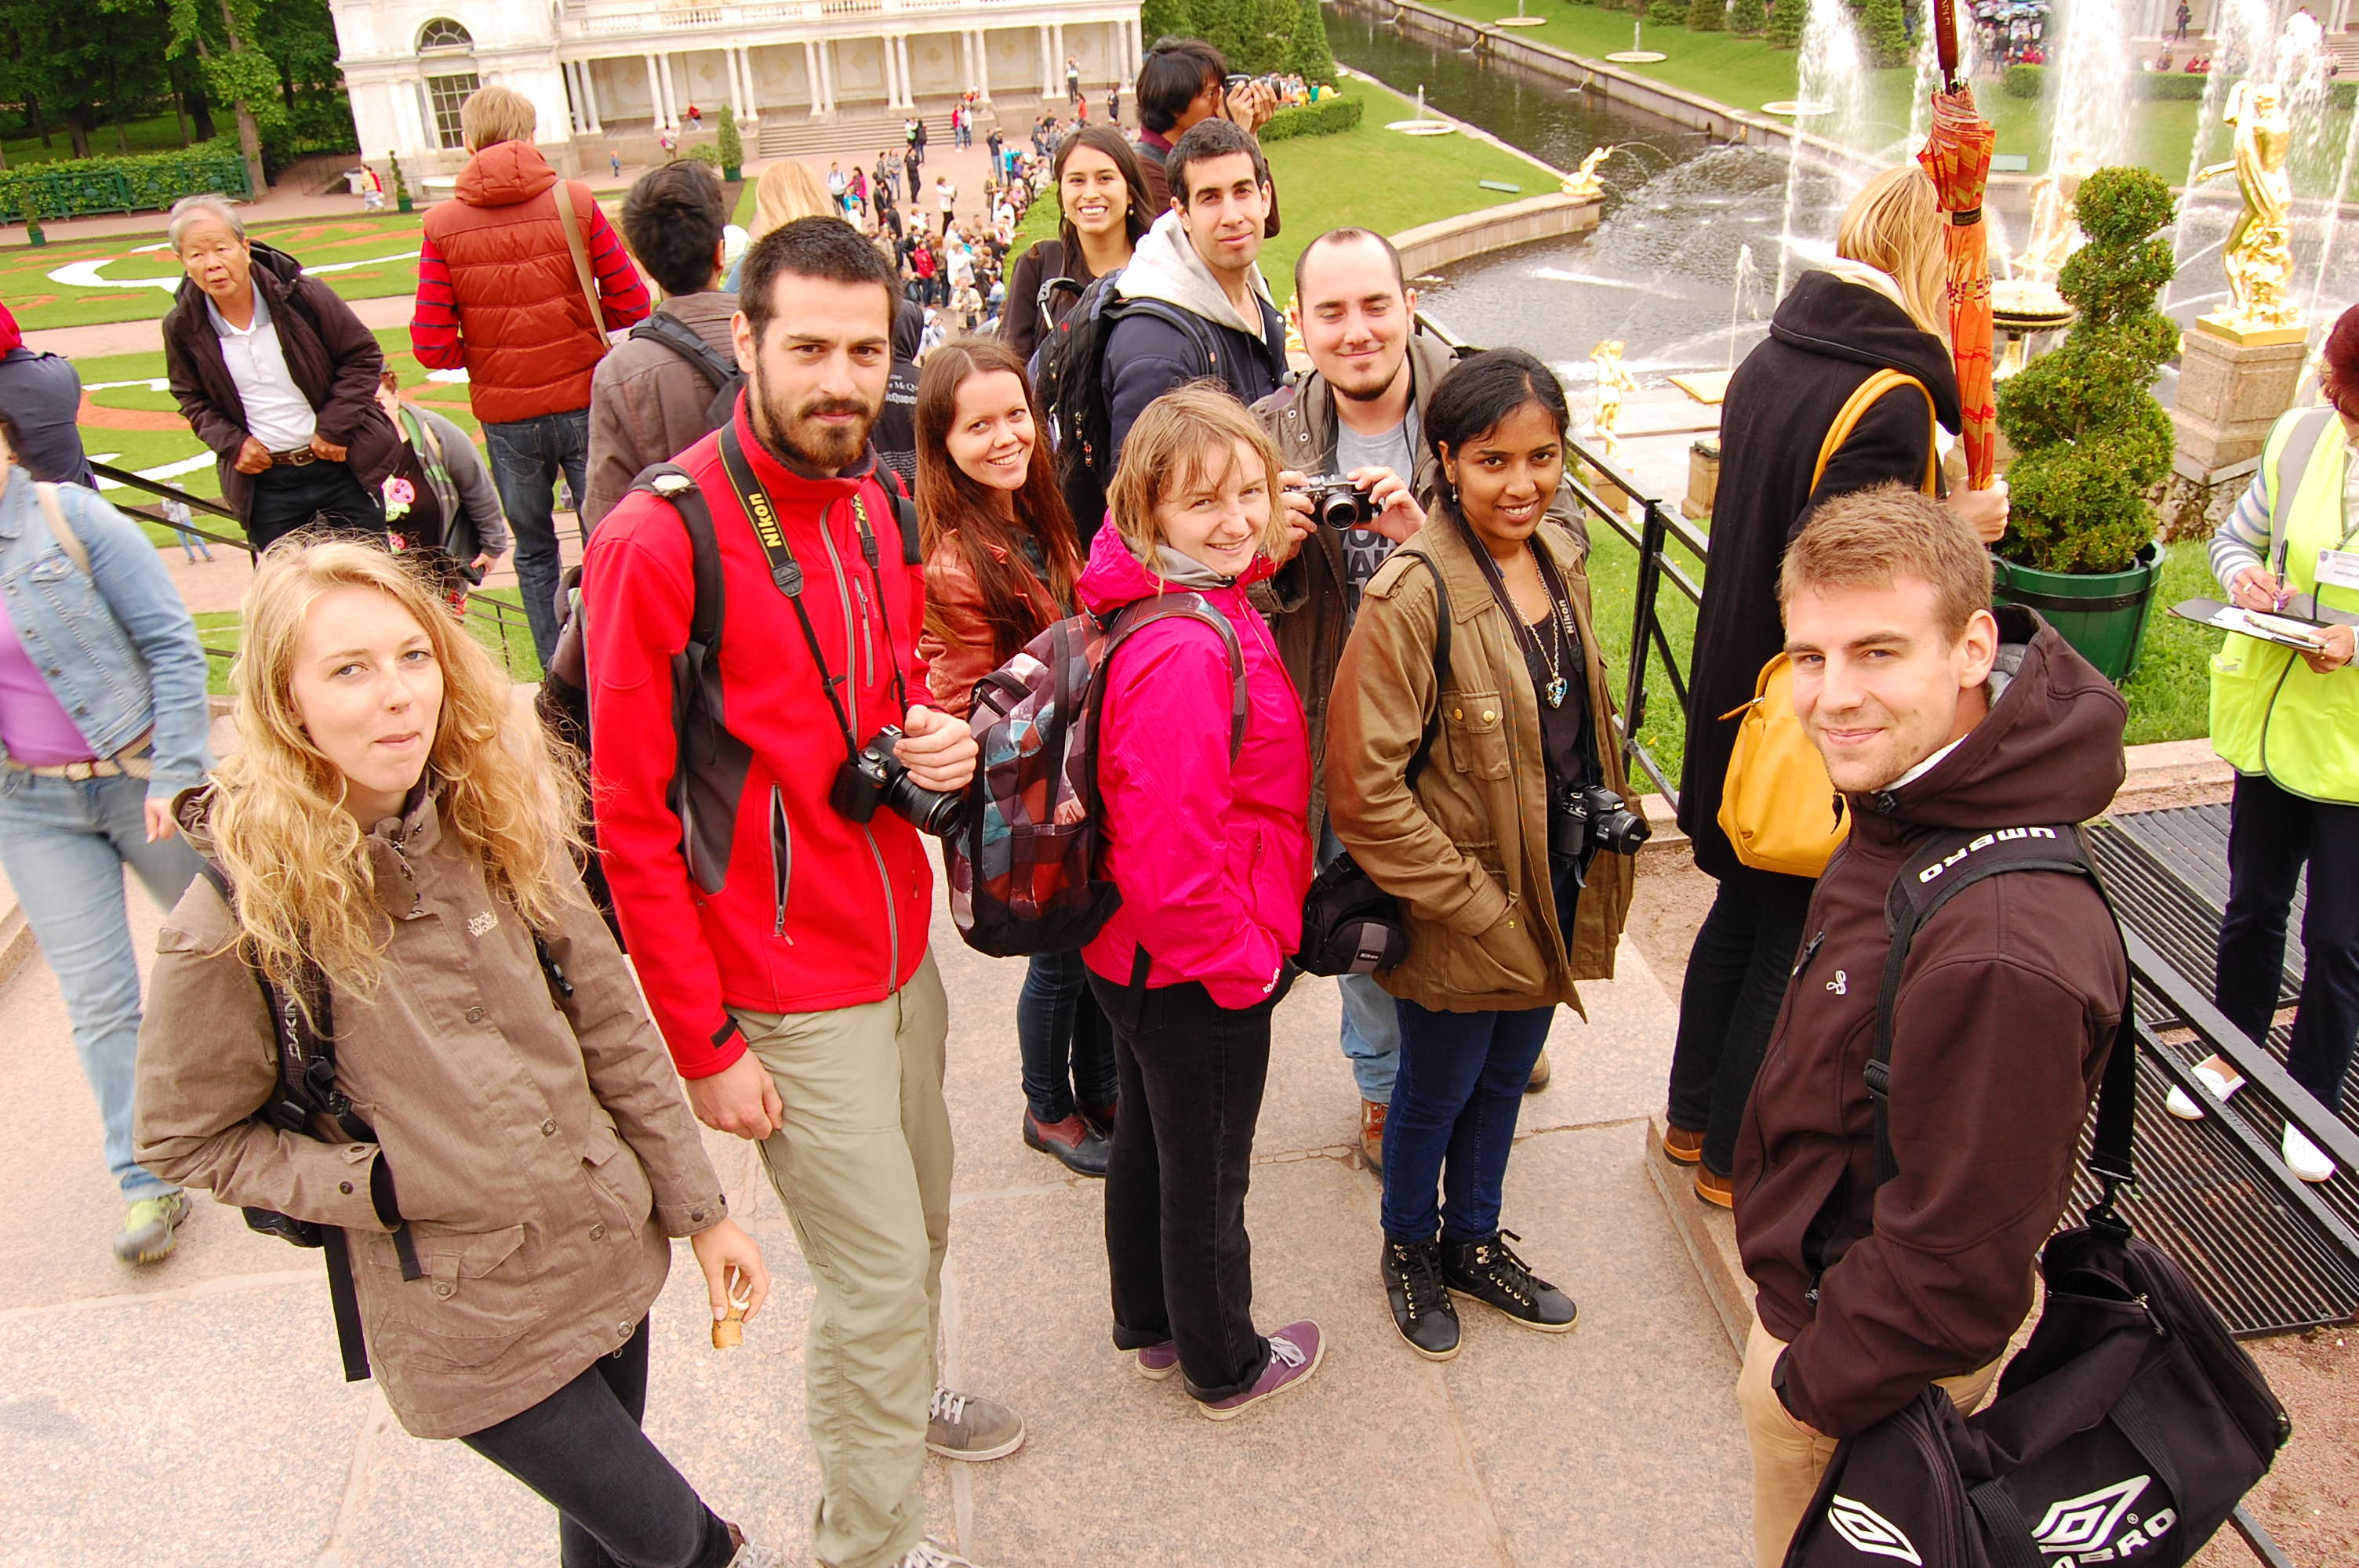
\includegraphics[width=0.45 \textwidth]{media/front_picture.jpg}
\\
\end{wrapfigure}
	
\NewsItem{Author's thoughts} % Main next item title
\vspace{3pt} % Some extra whitespace since there is no author as for the news in the body of the newsletter
\textit{
%12345678901234567890123456789012345678901234567890123456789012345678901234567890
Before going abroad, to pursue my master's degree, I was living in little 
paradise called Cyprus. 
A sandy island in the Mediterranean sea surrounded by three continents, 
offering strong sun light most of the year, amazing beaches, kind and friendly people 
with great hospitality, chill and easy going life-style. 
However, the world was much bigger and attractive, in many and different ways, than 
I initially thought.
Once I visited four different countries, in the context of my studies, I came to 
realise that I have only read a chapter of this book called ``Our World''. 
I never thought before that: travelling; meeting new people; learning new things; 
accepting facts and mentalities from different cultures; will be an exciting and 
a large part of my daily life. 
I have met people who gained my utmost trust and respect, and no matter how far 
away they are now they are still close and always in my thoughts.   
And one thing I know for sure, I would never have been the person that I am today 
if I hadn't take the big leap and exit my comfort zone.
}
\par\hfill --- Stefanos Georgiou
\end{minipage}
\end{center}

\vspace{0.5cm}
\SepRule % Small horizontal rule after the main news item
\vspace{0.5cm}

%\setlength{\columnsep}{16pt} % Uncomment to manually change the white space between columns
\begin{multicols}{3} % Begin the three-column layout

%----------------------------------------------------------------------------------------
%	OTHER NEWS
%----------------------------------------------------------------------------------------

\NewsItem{What was I thinking?}
\NewsAuthor{Stefanos Georgiou}

%12345678901234567890123456789012345678901234567890123456789012345678901234567890
Growing in a small island (\textit{i.e.} Cyprus), I had a limited knowledge regarding 
the vast experience, new ideas, and cultural benefits I could assimilate while 
travelling abroad. 
Being in the last year of my under graduate studies, at the University of Cyprus, 
I had an aim of doing my post graduate degree in United Kingdom or any other 
English speaking country. 
In addition, alongside with the University, I had full time barman responsibilities 
at Starbucks cafeteria to collect money for my studies. 
While being in a family of six, with four siblings, I believed it was important 
to get funds by any means to reduce the burden on my parents for doing my post graduate 
degree. 
The opportunity was given, to do my studies, while being eligible and qualified to 
receive a Erasmus Mundus scholarship, after I applied for {\sc perccom} (PERvasive 
Computing and COMmunications for sustainable development) program. 
A fact that made me super happy and left a huge smile on my face for many days.


%12345678901234567890123456789012345678901234567890123456789012345678901234567890
The above-mentioned master program offered studies with the subject of GreenIT and 
sustainable development with the opportunity of studying in four different counties 
(France, Finland, Russia, and Sweden) for 18 student for the duration of two years. 
Moreover, it was a unique chance to meet people from different cultures and backgrounds 
since it was an international program and one of its purpose was to bring together 
students from various countries. 
However, a bit skeptical about this choice, as a person who never lived abroad and 
who do not even know how to cook, I took the decision for exiting my comfort zone 
and in September of 2013 I started my studies abroad. 
But who would know that I will end-up addicted in living abroad and having the 
travelling aspect as part of my life?


%12345678901234567890123456789012345678901234567890123456789012345678901234567890
During these two years of my post graduate studies, I acquired knowledge and 
experience that I would never had if I only stayed in a tiny island. 
My purpose is to share and motivate young people to get out of their comfort zones, 
travel a lot without thinking too much, meet a bunch of crazy people with no limits, 
and never forget to take your smile whenever you go or whatever the situation it is.

%-----------------------------------------------------------
\NewsItem{First stop: France}

%12345678901234567890123456789012345678901234567890123456789012345678901234567890
France, the country of great wines, delicious cheese, funny English accent, 
and kind people was the first stop of my studies. 
More specifically, the city Nancy (located in the Northern France) offered its hospitality 
for the 18 {\sc perccom} students. 
The dream team composed from three French, two Nigerians, two Indians, two Bangladeshi, two 
Indonesians, a German, a Peruvian, a Ukrainian, a Romanian, a Vietnamese, and a 
Cypriot/Hungarian (myself).  


\begin{center}
	\includegraphics[width=0.32\textwidth]{media/strasbourg.jpg}
	\par\textit{City of Strasbourg}
\end{center} 

%12345678901234567890123456789012345678901234567890123456789012345678901234567890
I arrived in Nancy late in the evening, being exhausted from the trip, sweaty and 
dirty, and more importantly super hungry! 
That was my first encounter with Fisayo Caleb Oluwagboye, a guy from Nigeria also 
a student in my program about the same age as I. 
A kind, smart, and quite person who is a very dear friend of mine 
and who later on asked me to become his best man for his wedding.    
Even now (years after my studies), we regularly speak over Skype, or we try to 
meet at least once a year. 
Long story short, he was the first person who cooked for my when I arrived in Nancy 
during that night once he realised how hungry I was. 
After that day we where always going out together, he was the person I trusted to 
speak my mind and the things that were bothering me like relationships, family staff, 
or studies. 


%12345678901234567890123456789012345678901234567890123456789012345678901234567890 
Our studies, in the University of Lorraine, where intense since we had to 
follow lectures eight hours almost every day. 
The French education system is build mainly from long hours of lectures and less 
load on homework. 
In addition, we had to speak formally with most of the professors compare to the 
Scandinavian Universities. 
We received most of the student guidance in the French Universities from our 
cohorts' students, Alexandre De Masi, Baptiste Louis, and Dorine Petit. 
Alexandre was our group's techno-freak, he was always connected and following 
every step of different technological advancements, but, mainly in the communications 
field. 
Baptiste was our group's \textit{princess}, a nick name that everybody liked and used. 
The nick name was given be me and Dorine while searching for a picture with the ``thank 
you'' description and the princess word was also written there. 
Dorine was our group's dance addict, she was always willing to help us while 
staying in France, and she was responsible for writing the {\sc perccom}'s blog and 
news.
These three were the people who mainly help us to bypass the hard French conversations 
in different domains. 
Also, they gave us the first flavour of France while partying and organising 
social events with them. 


\begin{center}
	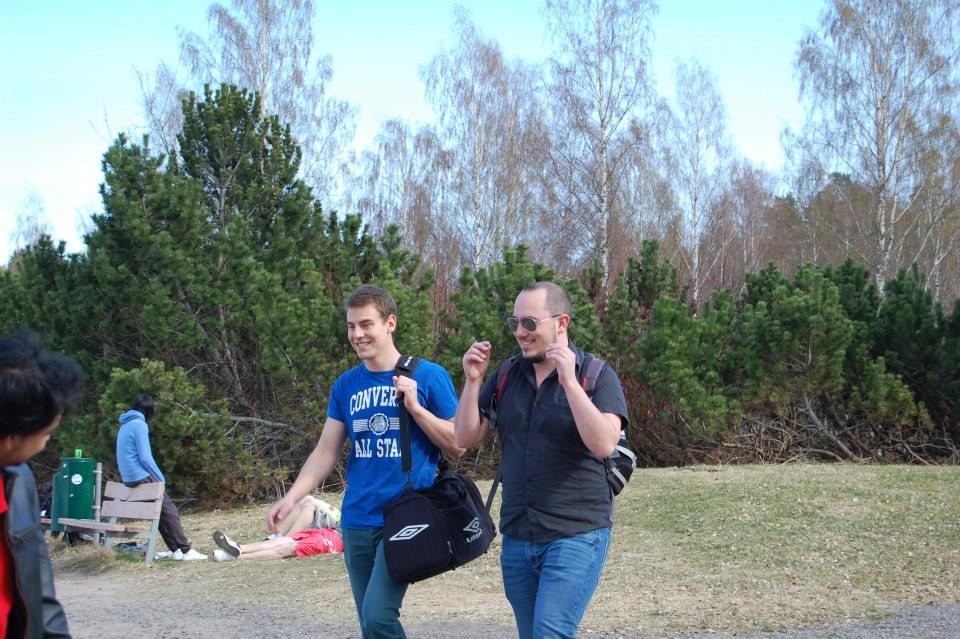
\includegraphics[width=0.32\textwidth]{media/baptiste_alex.jpg}
	\par\textit{Baptiste and Alexandre}
\end{center} 


%12345678901234567890123456789012345678901234567890123456789012345678901234567890
During our stay in France, our program organised trips such as visiting winery 
villages where the French speciality lies. 
These are amazing places to get tipsy while testing the different variations 
among the most excellent wines from years of knowledge that France has. 
The locals tried to help us to understand what are the differences of a good wine 
and how we should handle it based on its age. 
For instance, you should be more gently and careful with handling old read wines
and less time is required to let it ``breathe''. 
We also learned that the difference of champagne against the other sparkling wines 
is nothing more than the production place, the region of Champagne. 
However, with our still immature and youngster nature we where only focus on getting 
drunk and having fun instead, I still feel lucky that I remember all the above 
information that I am currently sharing. 


\begin{center}
	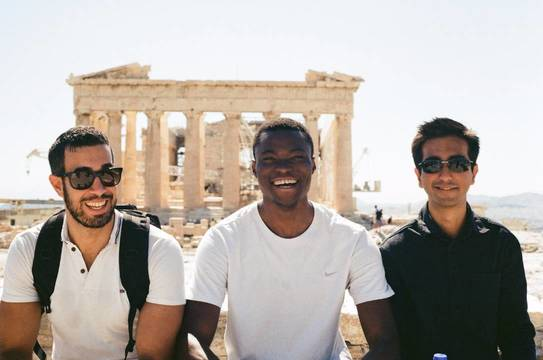
\includegraphics[width=0.32\textwidth]{media/stef_fisayo_rohan.jpg}
	\par\textit{I am left, Fisayo mid, and Rohan right}
\end{center}


%12345678901234567890123456789012345678901234567890123456789012345678901234567890
Another great experience that we had in France was the international evening 
we organised among the {\sc perccom} students at Alexandre's apartment. 
The aim was to bring traditional food and alcoholic drinks from our home countries 
and let everyone to have a taste from it. 
We tasted food from approximately eleven various kitchens, the apartment of our 
host had smells from different spices and food for at least a week. 
I guess these smells also disturbed Alexandre's sleep since for some time he look 
really sleepy, or maybe it was the intense courses from our University with the 
combination of French professors accent while trying to teach in English.  
Nevertheless, we extended the night by having some beers at a local pub. 
As a non-beer drinker, I decided to try one, however, the options were various 
and all unknown to me. 
That was the time when one of our fellows, Vlad (Romanian scout guy who was wearing a 
red characteristic jacket, drinking beers like water, and skilful programmer), 
told me the fantastic quote that I even use nowadays. 
\textit{``Stefanos, when you don't know which one to pick just go for the blondes, 
	they are always a good choice''.} 
By thinking of that quote again, I am not aware if he only meant that for beers.


%12345678901234567890123456789012345678901234567890123456789012345678901234567890
The first semester was quite fruitful for me in both terms of education and 
life experience since I have done new thing like basic French conversation, 
activating my apartments fire alarm a couple of times while cooking, building home 
automation systems for smart houses and so on. 
After an awesome first semester in France, we packed our stuff and travelled 
to our next destination, the ice-cold Lappeenranta of Finland.


%-----------------------------------------------------------
\NewsItem{Second stop: Finland}

%12345678901234567890123456789012345678901234567890123456789012345678901234567890
The country of the thousand lakes and two millions of saunas is Finland. 
Where people are quite, peaceful, barely speaking to strangers, not making eye 
contact, and they feel you are inviting their personal space if you stand too 
close to them. 
However, when they start drinking alcohol and partying they become open and cheerful. 
   
\begin{center}
	\includegraphics[width=0.32\textwidth]{media/entrance_university.jpg}
	\par\textit{Lappeenranta University's entrance}
\end{center}
   
%12345678901234567890123456789012345678901234567890123456789012345678901234567890 
In the beginning of January 2014, Finland welcomed our cohort with snowy days 
and long nights. 
In the north, most of countries have long nights during winter times and long 
days during the summer times. 
Some common patterns of the Scandinavia countries are: sun is rare and a valuable; 
prices of alcoholic and cigarettes are high due to taxation; eating in a 
restaurant is pricey; expensive bus tickets; getting a descend hair cut costs; 
high education and well structured system; amazing public health service; buses on time; 
and every single person knew English and with a proper accent.


%12345678901234567890123456789012345678901234567890123456789012345678901234567890 
To reduce some of these aforementioned costs since we had a small scholarship and 
definitely not one that is enough for Scandinavian countries, we took some 
necessary steps. 
For example, we bought a complete hair cut kit and we entrusted out hair to 
Alexandre---who only had experience in trimming sheep's fur as one time he said 
while being tipsy.  
Worth to say for free hair cut it wasn't that...bad! 
For reducing the transportation fees, since I was leaving five kilometres away from 
the University, I used to walk everyday. 
Luckily the lake Saimaa, the one I had to pass by to get at the University, got 
frozen. 
Therefore, it offered a direct part to the University if someone was crazy enough 
to risk working on the frozen lake. 
However, a bit uncomfortable initially---because as a Cypriot I am only experienced 
on walking on the sand or swimming in sea---I took the big step and started everyday 
going to the University through the frozen lake.
This brave decision of mine reduced the walking time, towards the University, from 
30 to 15 minutes.


\begin{center}
	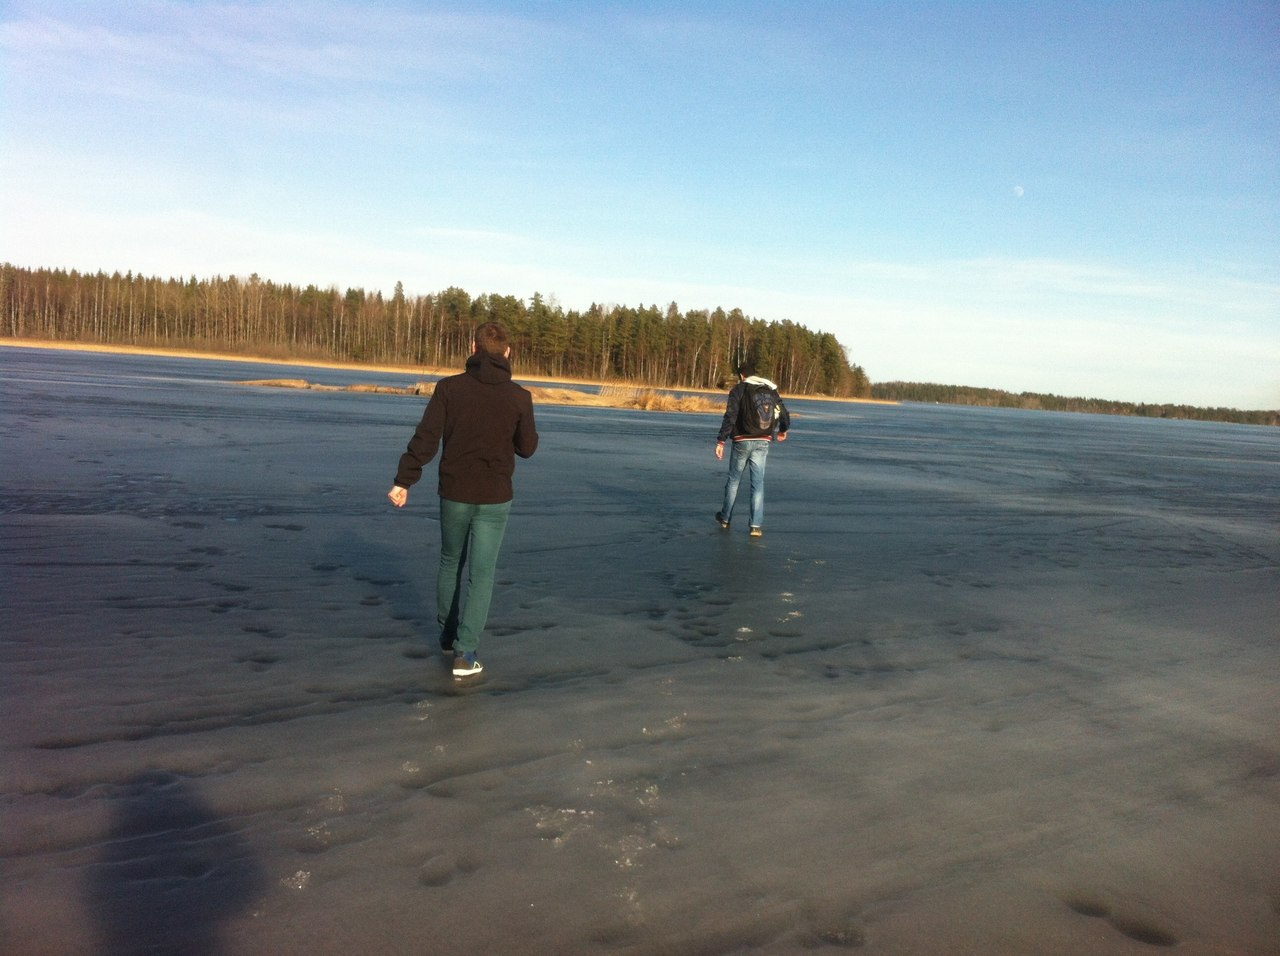
\includegraphics[width=0.32\textwidth]{media/walking_on_ice.jpg}
	\par\textit{Walking on a frozen lake to go home}
\end{center}


%12345678901234567890123456789012345678901234567890123456789012345678901234567890
Regarding the Finish education system, is consider to be one of the most successful 
one. 
Some key factor to their success is the reduced lecture hours and the increased 
load on homework. 
In addition, most of the Finnish students do not study more than eight hours, 
University's lectures included as studying hours. 
They are trying to keep a balance between studies and student life instead of 
spending endless hours at the University. 
Also, the Finish Universities are open 24/7 without any guards and student can 
access different parts of it while using their student cards. 
Moreover, students can book different classes, meeting rooms, and saunas 
in the University to organised social events like project meetings or even parties. 
In our cohort the main organiser of the {\sc perccom} parties and our ambassador was 
Vicky Palacin Silva. 
A crazy Peruvian girl who has unlimited source of energy and patients, great 
organising skills, and who is always in party mood. 
Also, no matter what questions we had, Vicky always knew or she could 
find the answers. 
Alongside with Vicky you could always find Vlad and Maike; a vegan German girl 
who I often used to teas with bad meat quotes and jokes, even tho we became 
great friend but I still teas her.


\begin{center}
	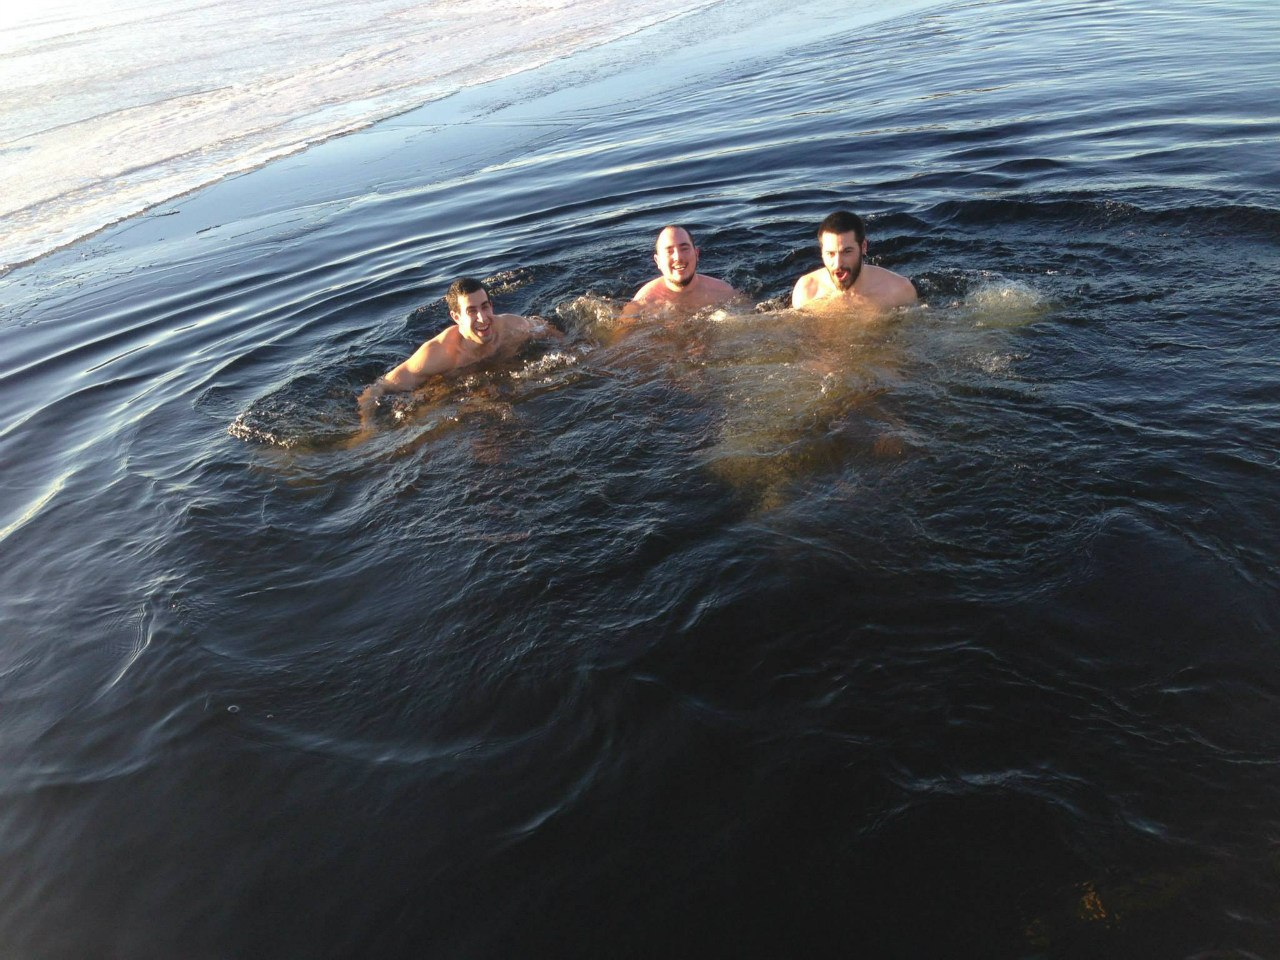
\includegraphics[width=0.32\textwidth]{media/after_sauna_lake.jpg}
	\par\textit{Jumping in a frozen lake after sauna}
\end{center}


%12345678901234567890123456789012345678901234567890123456789012345678901234567890
Sauna is undoubtedly one of the most serious social events in Finland since business 
man can close deals there with just a simple handshake. 
For Finish people giving your word that you will do something is serious. 
In addition, Finland has five millions of population and two million of saunas. 
Most to the buildings offer sauna facilities and it is a habit followed by Finns 
very frequently during the week. 
We had also adopted this habit and we even tried the most extreme types of after 
sauna, like jumping in the snow or in a barely frozen lake. 
If anyone thinks that your body can withstand the cold lake of 2-3 degrees just 
because you where in the sauna where the temperature is around 80 is mistaken. 
The experience was freezing of course since we were running immediately back to the 
sauna after jumping in a cold lake.  


%12345678901234567890123456789012345678901234567890123456789012345678901234567890 
During the summer period, in Finland, the days are longer and as an outcome we 
experienced only four hours of night time. 
This is usually the perfect period of the year to start social events such as 
barbecue and parties near lakes until late hours. 
However, be advised that summer in Finland is not like a regular Mediterraneanise's 
country. 
It can even snow in May! 


%12345678901234567890123456789012345678901234567890123456789012345678901234567890 
By the end of the second semester, we had a two weeks of seminars in one of our 
partners University, the {\sc itmo} University of Saint-Petersburg. 
To this end, we packed our luggage for the next adventure by the middle of May 
in 2014.	

%-----------------------------------------------------------
\NewsItem{Third stop: Russia}
%  
%12345678901234567890123456789012345678901234567890123456789012345678901234567890 
\textit{``When will we reach the Russian boarders"}, was my first question, while 
travelling to Saint-Petersburg by bus, towards our Ukrainian fellow Vitali 
Poliakov  (another techno-freak, that you can align with Alexandre De Masi, 
combined with the slow eating behaviour, his usual quote 
\textit{``no no stop stop stop"}, and his unique surprise expression very time 
he sees something odd). 
Vitali then took his serious expression and said \textit{``You will realise it 
	because your ass will start hurting from the bumpy road"}, he said. 
I could not agree more, the bumpy road combined with the strict check-up of 
passports and languages was our welcome ceremony to Russia.


\begin{center}
	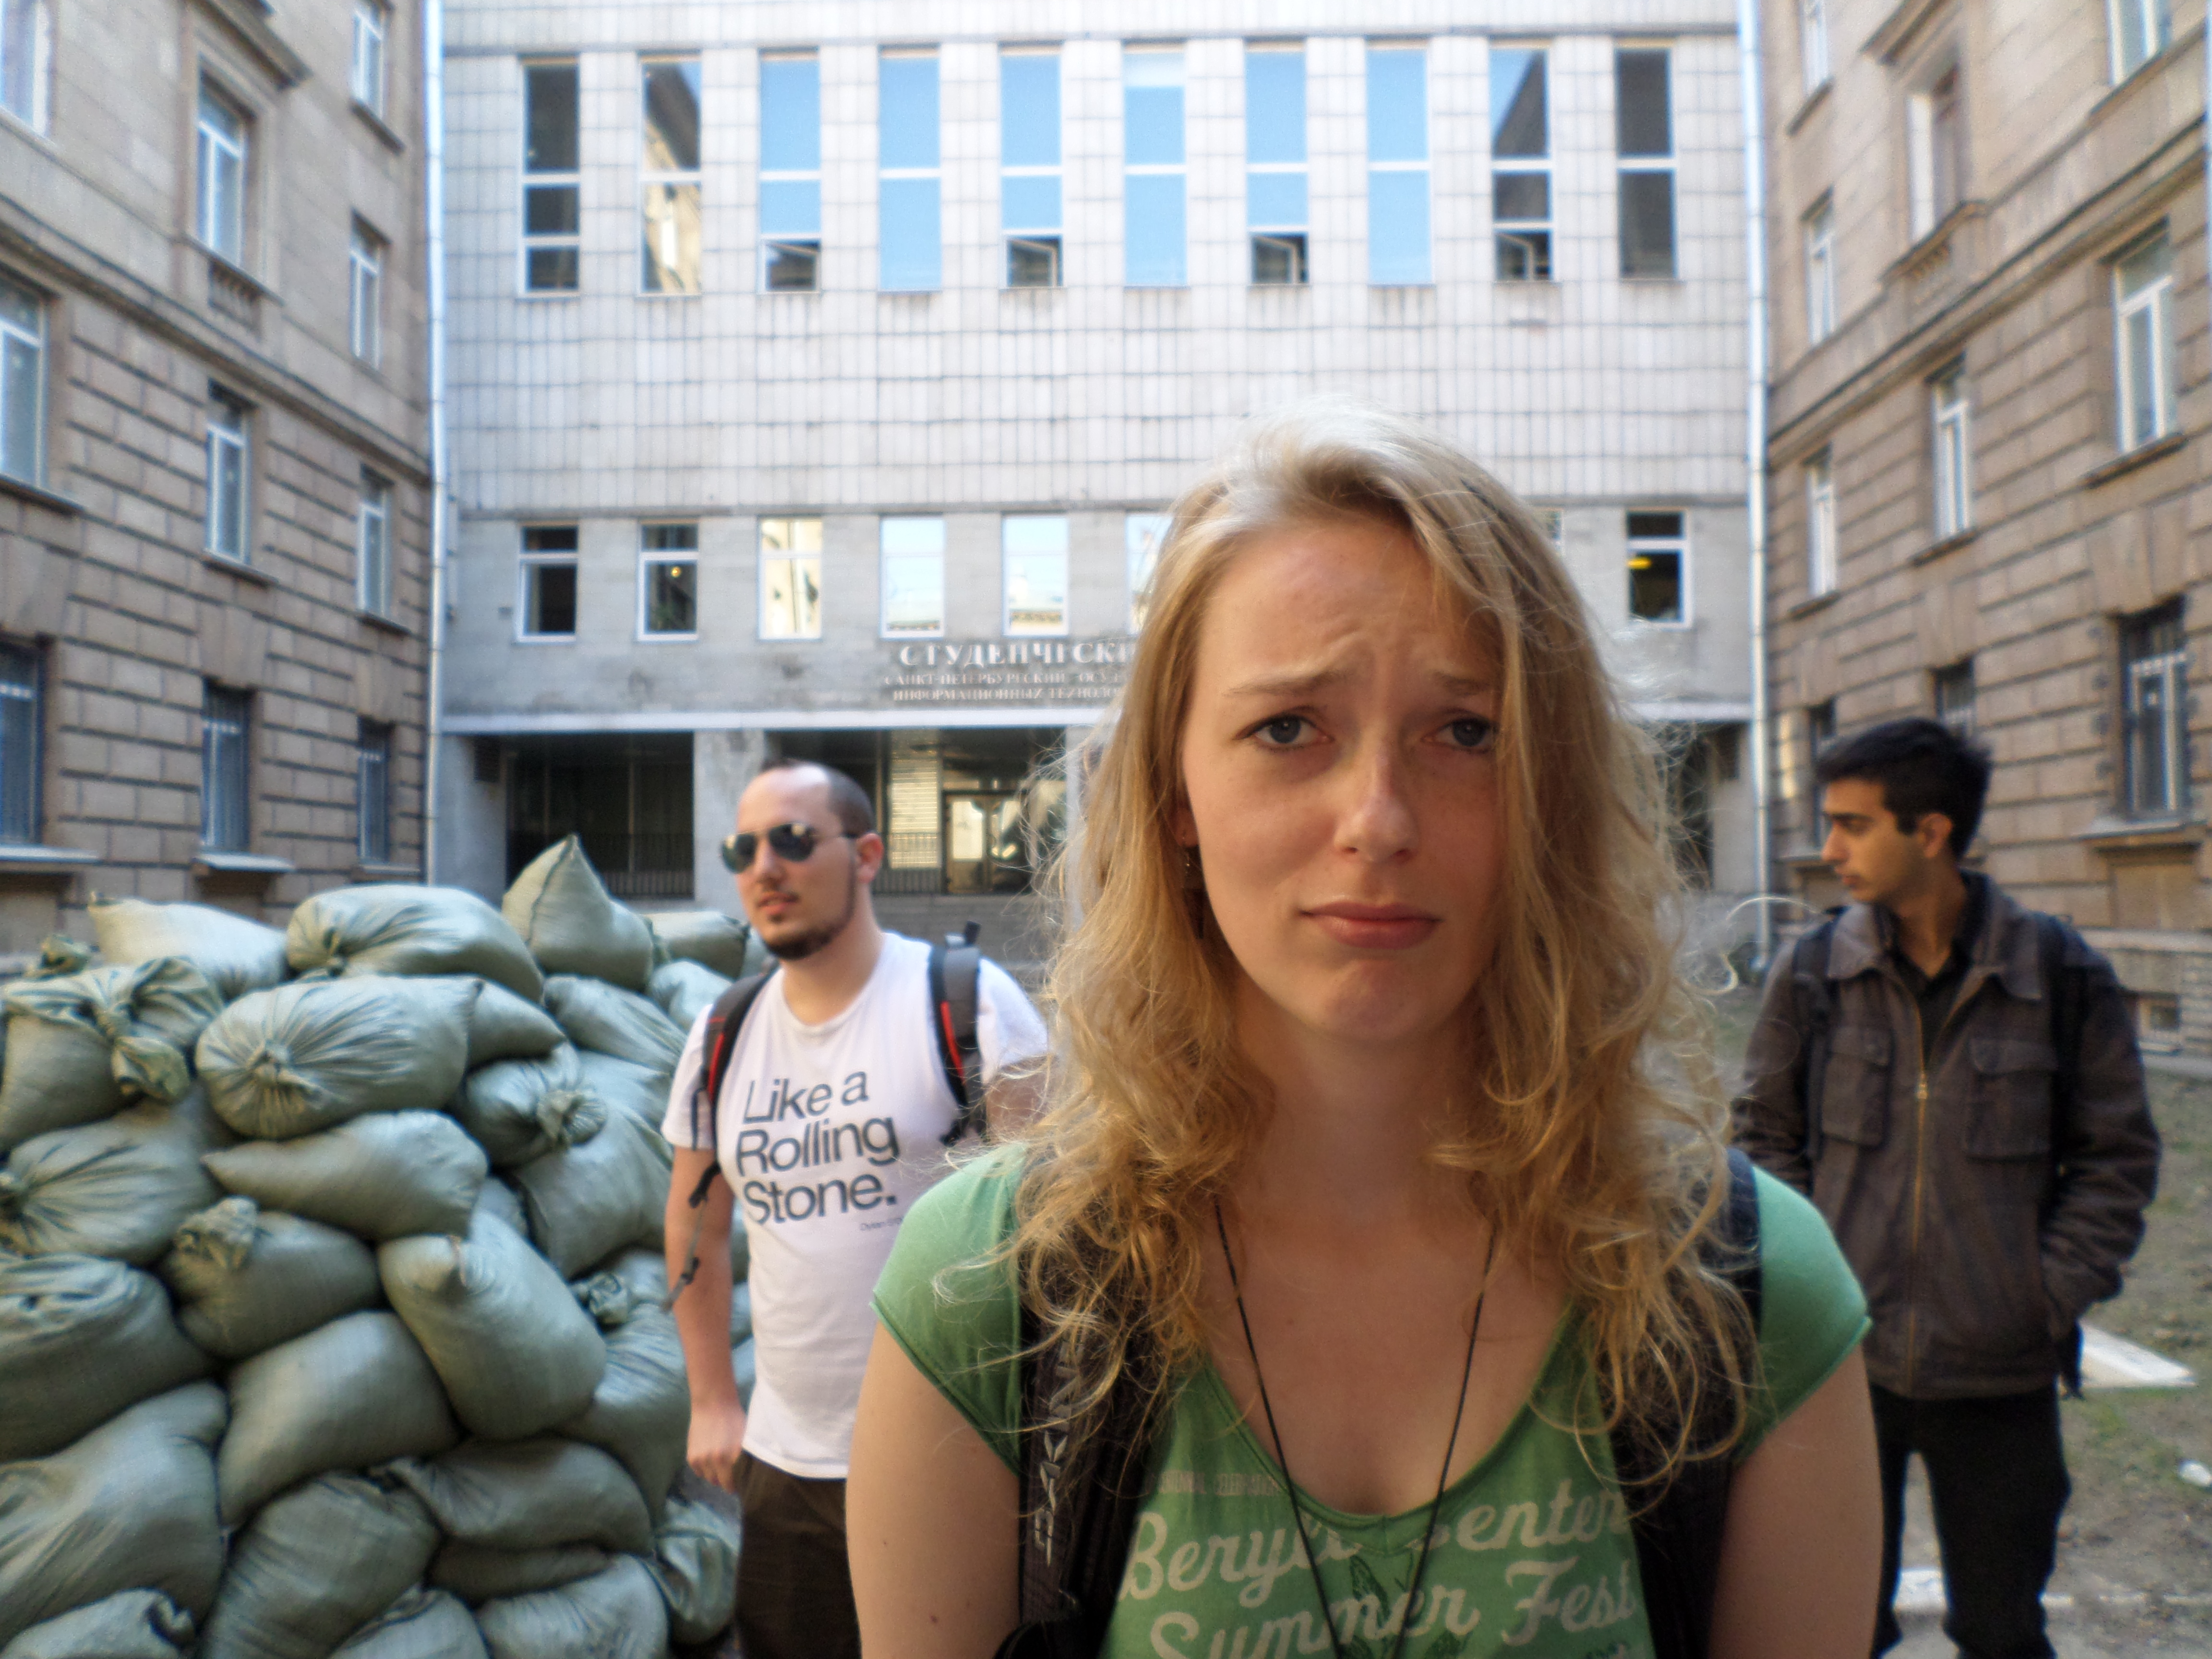
\includegraphics[width=0.32\textwidth]{media/accommodation_in_spb.jpg}
	\par\textit{Maike's face for our accommodation}
\end{center}


%12345678901234567890123456789012345678901234567890123456789012345678901234567890
During the first day, Saint-Petersburg's beauty was hidden from us by the cloudy, 
moody, and rainy weather, a fact quite usual for this city even during summer time.  
Nevertheless, the combination of the neo-classical architecture, bridges, monuments, 
theatres, operas, and ballets are giving the city a beautiful, attractive, 
and cultural view. 
In addition, the party places, cafeterias, and restaurants, that vary in the 
city, are providing a comfort and many options for its locals and tourists. 


\begin{center}
	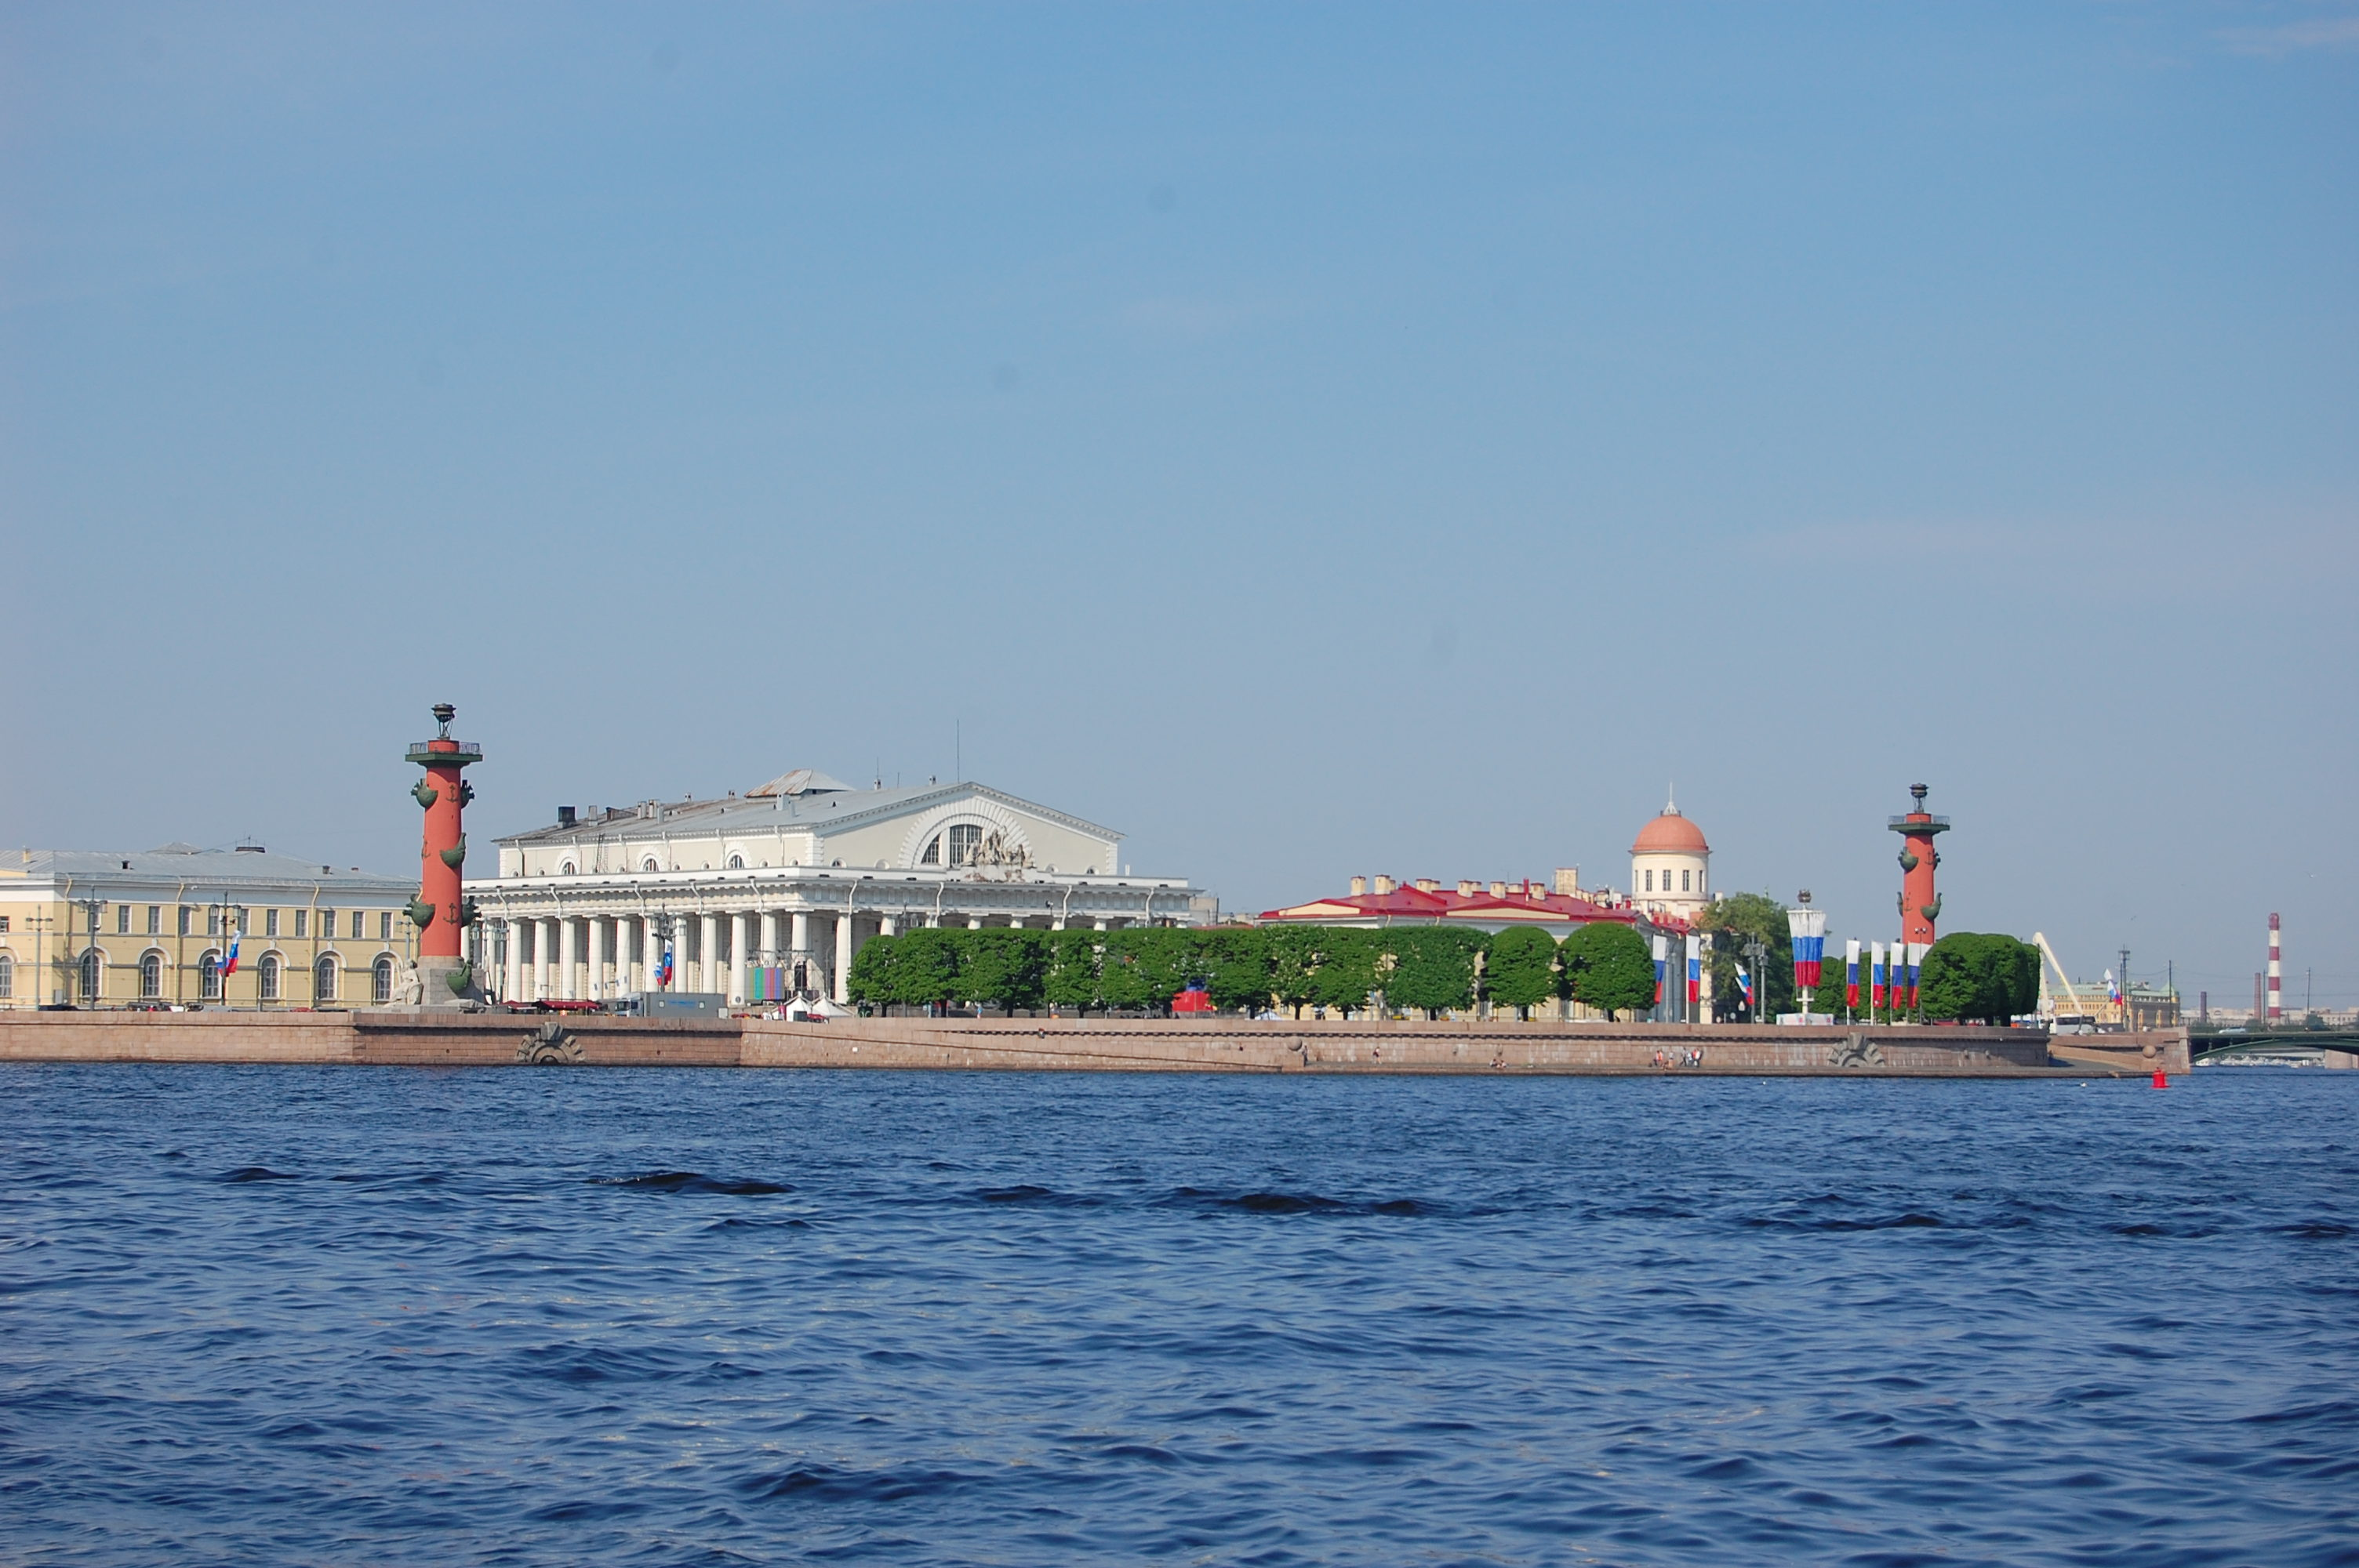
\includegraphics[width=0.32\textwidth]{media/spb_1.jpg}
	\par\textit{Vasiliovsky island}
\end{center}

%12345678901234567890123456789012345678901234567890123456789012345678901234567890
The expression on Maike's face (see first picture) about our accommodation was 
priceless. 
The dormitory had a lot of sand bags packed in the entrance and high iron gates; 
which made it look like a war zone.  
In addition to that, four old Russian ladies were guarding the reception and 
monitoring every movement in the building. 
At every wrong action, like coming back at the dormitories late night, they 
were taking an angry look and start shouting some unknown Russian words to us. 
However, small daily actions such as smiling and greeting them in their native 
language contributed in a very friendly behaviour later on.


%12345678901234567890123456789012345678901234567890123456789012345678901234567890
Our hosting University, {\sc itmo}, had a research centre at Vasilievsky island 
next to the State University of Saint-Petersburg, where the current Russian 
president (Vladimir Putin) graduated. 
The seminars took place at the above-mentioned research centre, a building that 
is mainly decorated by marble, a circular stair case, 
and mosaics that gives a flavour of classical style. 
Same fact goes for almost all metro stations in the city, they look like 
museums covered with mosaics and marble pillars. 

 
%12345678901234567890123456789012345678901234567890123456789012345678901234567890
An interesting event happening in Saint-Petersburg during June are the white nights.
The outcome of this event is having day light all time long even during night 
time. 
Something that caused me confusion for many days since most of time I could not 
distinguish if it morning or night time. 
Sleeping masks or tick curtains are necessary if you end up in Saint-Petersburg 
on that period of time. 
The white nights are starting on 11th of June and last until 2nd of July.
In addition, during summer time, when the ice in the Neva river is melt (river 
connected with the Finnish Gulf), the bridges are rising to pave paths for the 
transport ships. 
Even tho it happens every year, you could still see many people standing by the 
river's embankment to view this event, listen to music played near the bridges by 
local musicians and to enjoy the moment.
 
 
\begin{center}
	\includegraphics[width=0.32\textwidth]{media/petergof.jpg}
	\par\textit{The summer palace, Peterhof}
\end{center}


%12345678901234567890123456789012345678901234567890123456789012345678901234567890
For our Master Thesis, we had to choose a topic of our interest during the first 
semester. 
The associated partner for my topic was {\sc itmo} University of Saint-Petersburg. 
A choice I believe it was the finest after experiencing for two week in that 
magical city.

%-----------------------------------------------------------
\NewsItem{Forth stop: Sweden}

%12345678901234567890123456789012345678901234567890123456789012345678901234567890
Sweden, the country where most of people are blonde with blue eyes, 
where \textit{fika} (a coffee break habit) is a mandatory after every lunch, 
even at fast food places. 
The country where our {\sc perccom} team experienced numerous hokey games, Northern 
Lights very often since our hosting University was located in the north (Lulea), and 
felt the freezing Swedish cold weather of minus \ang{30}. 
Also, compared to Finland, Sweden is still very expensive and the student housing is 
a mess since there are not enough facilities to host all students. 


%12345678901234567890123456789012345678901234567890123456789012345678901234567890
Since Lulea is located in the far north of Sweden, we had often the opportunity to 
see the Northern Lights. 
Northern Lights is a beautiful view of the sky and there is a need of certain 
conditions to experience it. 
For instance, it shouldn't be very cold or windy, also it is far more clear and visible 
when there are no city lights close to it. 
In this line, many teams are organising the so called \textit{``Aurora hunting''} 
where they travel in the North of Sweden, places distant from cities, to experience 
the full view of the Northern Lights. 
I had the opportunity to see them a couple of times from my apartment's balcony. 
It never stopped to amaze me, every time I was just starring the view with silence 
and respect towards this world's wonder.



\begin{center}
	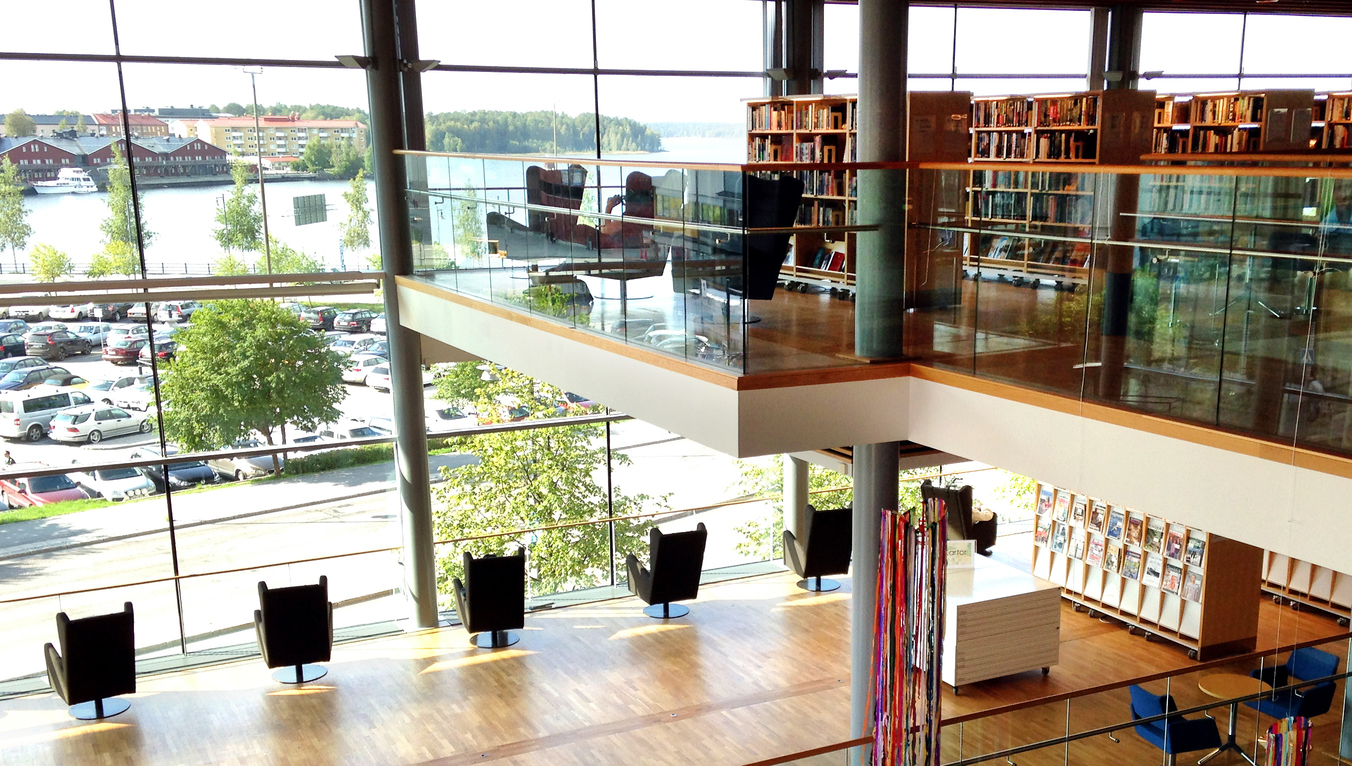
\includegraphics[width=0.32\textwidth]{media/cultural_centre_lulea.jpg}
	\par\textit{Cultural centre and library\footnote{retrieved from http://www.arcticairlink.com/kulturens-hus-in-lulea-where-business-and-culture-meet/}}
\end{center}

%12345678901234567890123456789012345678901234567890123456789012345678901234567890
Housing in Lulea was hard, since houses are limited for the large amount of 
students in the city. 
For the first month, me and a friend of mine, Iqbal Ahmend, we rented a cottage 
that was ten kilometres outside the city next to a beautiful forest and lake, and 
had a terrible internet access. 
Also, the bus schedule was very spare and from time to time we had to wait more 
than two hours (changing buses) to go from the University to city centre and then 
back to our cottage. 
However, after the first month we successfully rented a big and beautiful apartment 
in the city centre just next to the city's cultural centre. 
The cultural centre was a magnificent four storey building that had modern architecture and 
a whole site was made by glass. 
This fact offered a beautiful view towards the Gulf of Bothnia from the top floor with 
a pleasant working environment for the University students. 
We used to go there regularly to study and discuss different working projects, ideas, plans, 
and we stayed for hours while enjoying the view.

%12345678901234567890123456789012345678901234567890123456789012345678901234567890
The Technological University of Lulea's campus composed from a number of old but 
beautiful buildings. 
The whole campus had its own underground tunnel system that was inter-connecting 
all the University buildings. 
This was done to help students from moving to different buildings during winter 
without the need of going outside. 
Also, in a similar manner to Finland, the University of Lulea offered 24/7 access 
to its facilities for the students, even in the library. 
One of our favourite facilities, in the University, was the {\sc stuk}. 
A place where many social events were organised and many parties took place.
Something very interesting about the parties in {\sc stuk}, every time a party 
was finished security personal was sharing anti-hangover pills at the exit. 
In the begging I didn't believe that these pills are working. 
However, I greatly 
utilise them during my party times in Saint-Petersburg in Russia (I was 
studying there during the next semester of 2015).



\begin{center}
	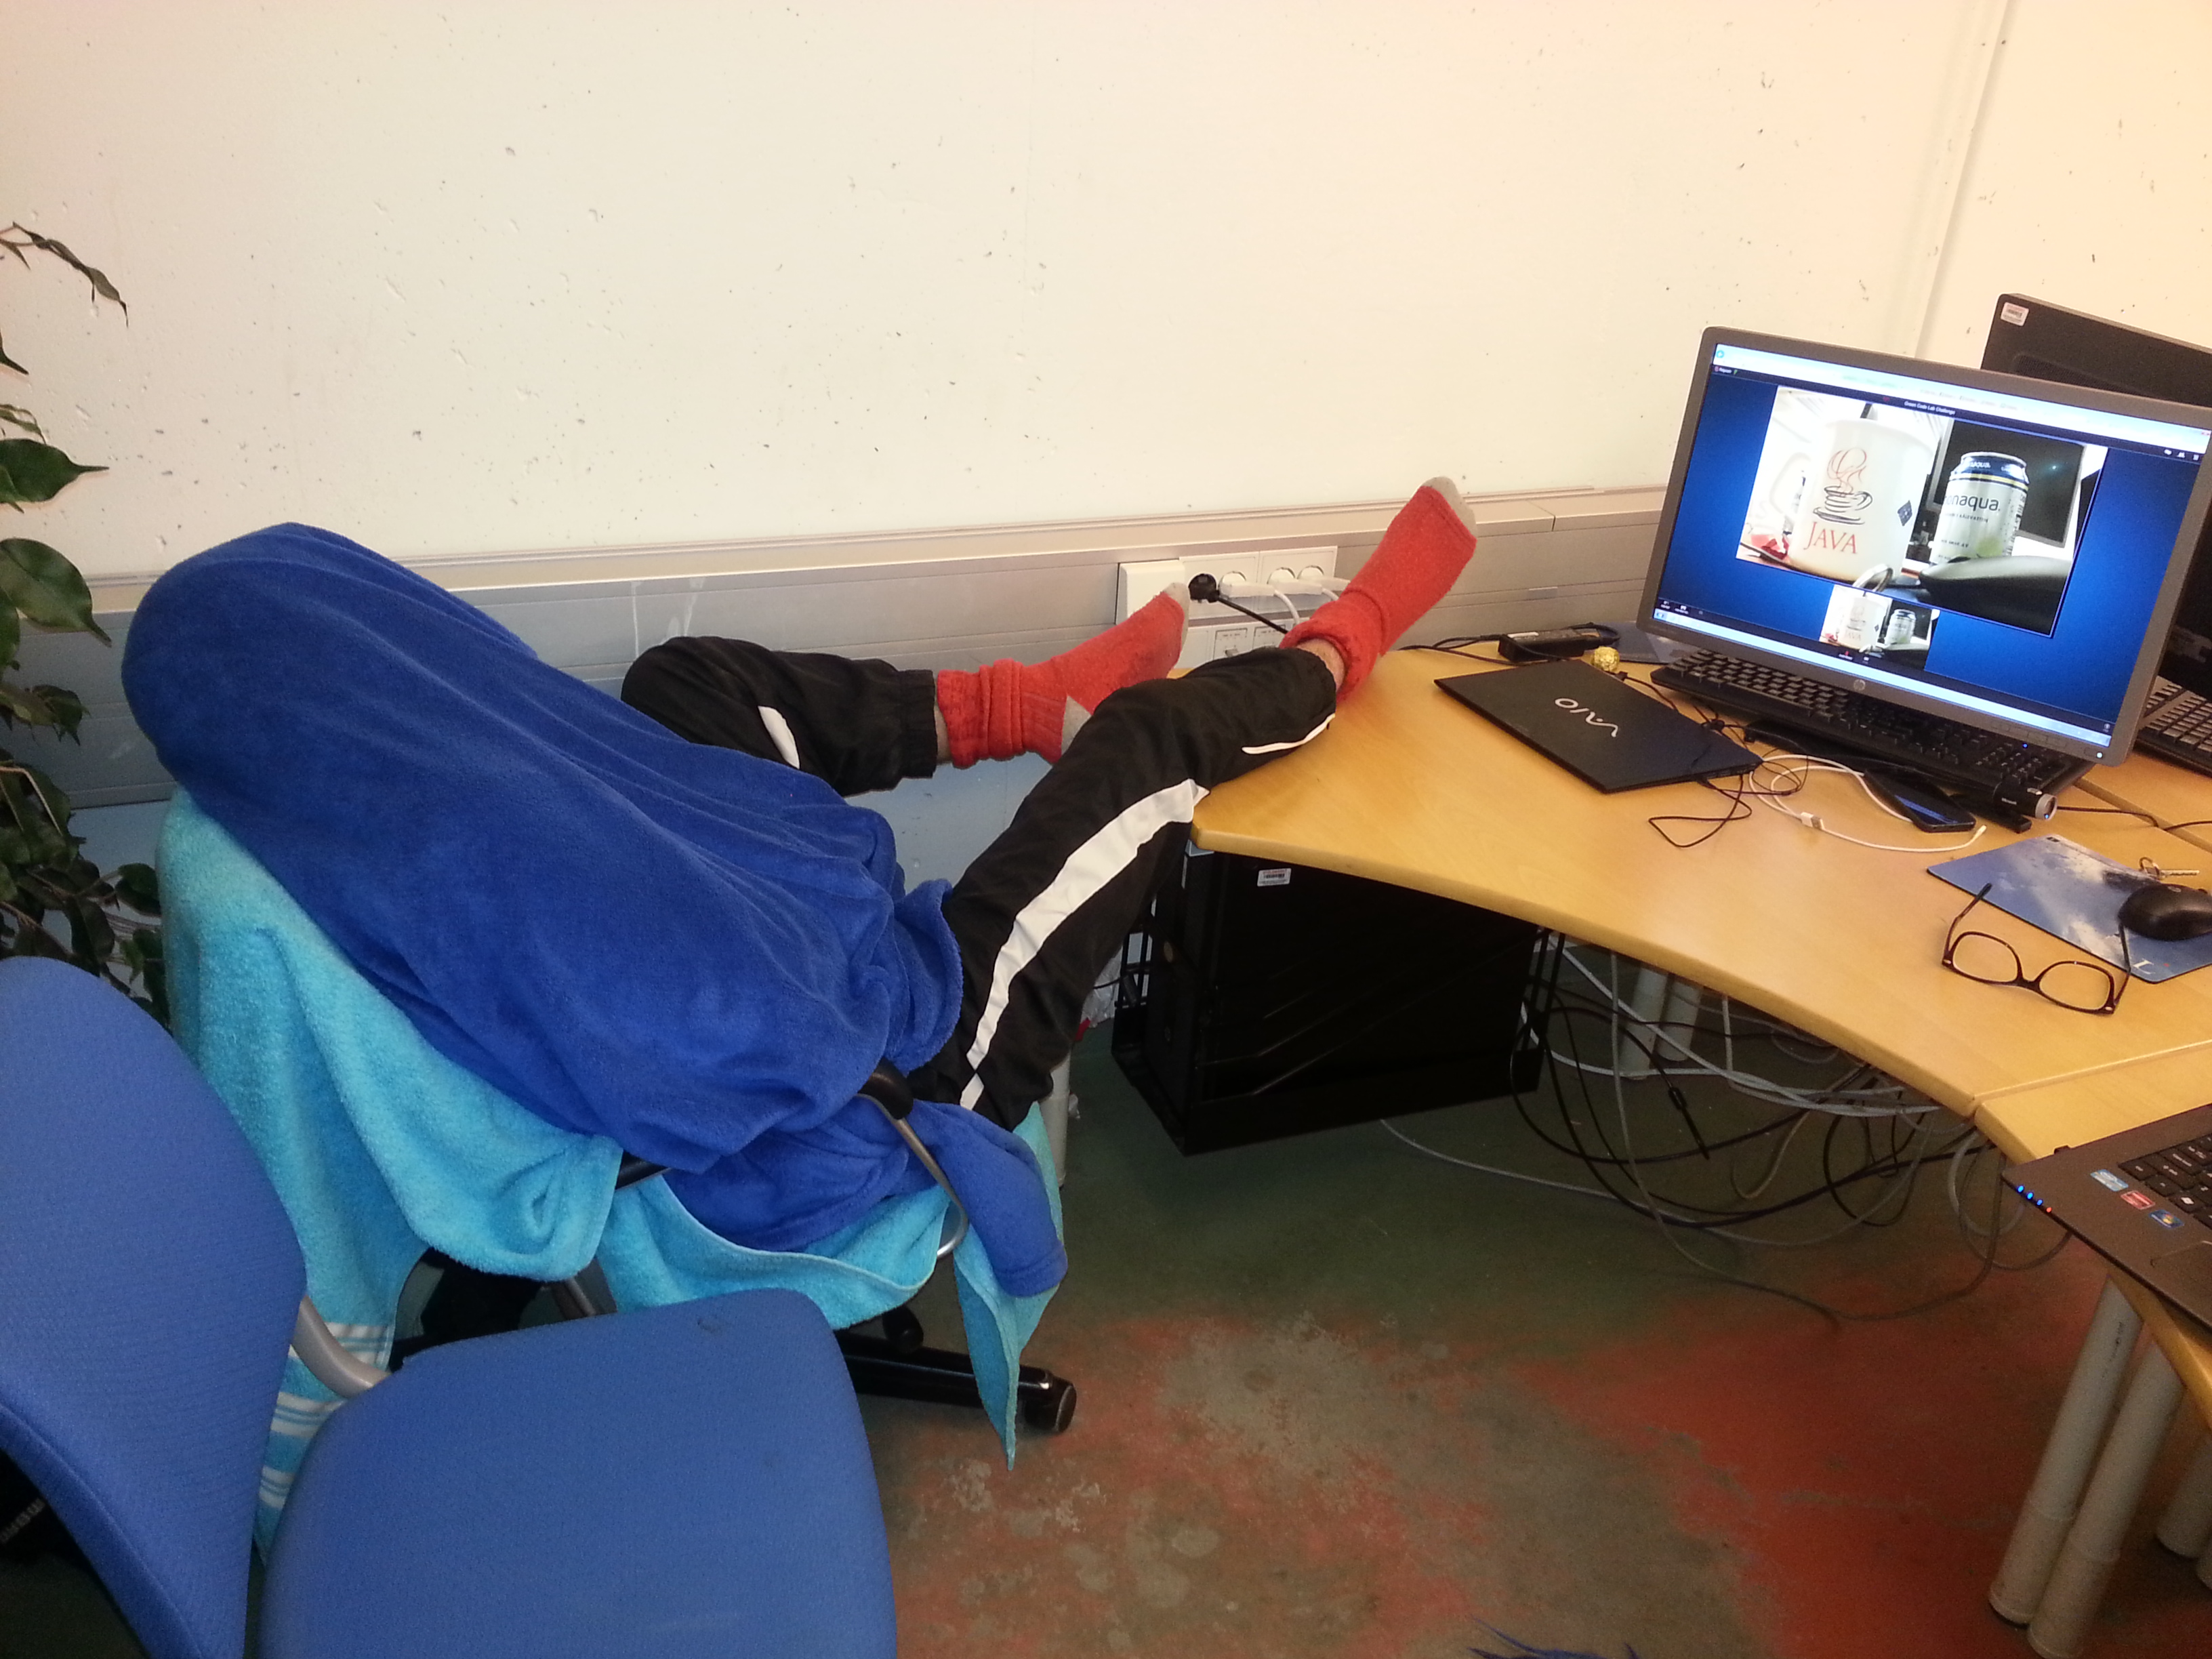
\includegraphics[width=0.32\textwidth]{media/coding_camp.jpg}
	\par\textit{Coding Camp, sleeping in the lab}
\end{center}
  

%12345678901234567890123456789012345678901234567890123456789012345678901234567890
Apart from partying and spending good time, we also took some challenges, in the 
context of our studies, such as the Green Coding Challenging Camp.
48-hours of non-stop and no sleep was my teams resolution for the above task. 
In my team, we had Baptiste as team leader, me and Zaine (a Nigerian girl with huge 
tolerance towards alcohol) as main software developers with two more students 
from a different cohort than ours who just started their post-graduate degree.  
We even packed our bags with my team, took our pyjamas, sleepers, towels 
(we were taking our shower at the University's gym) and we had as a collaborator an 
unlimited access to coffee machines and meals from Professor Karl Andersson every 
day. 
It was a crazy experience and a one I wouldn't do again sleepless. 
Nevertheless, the gains we got in terms of team collaboration and coding were 
priceless. 


\begin{center}
	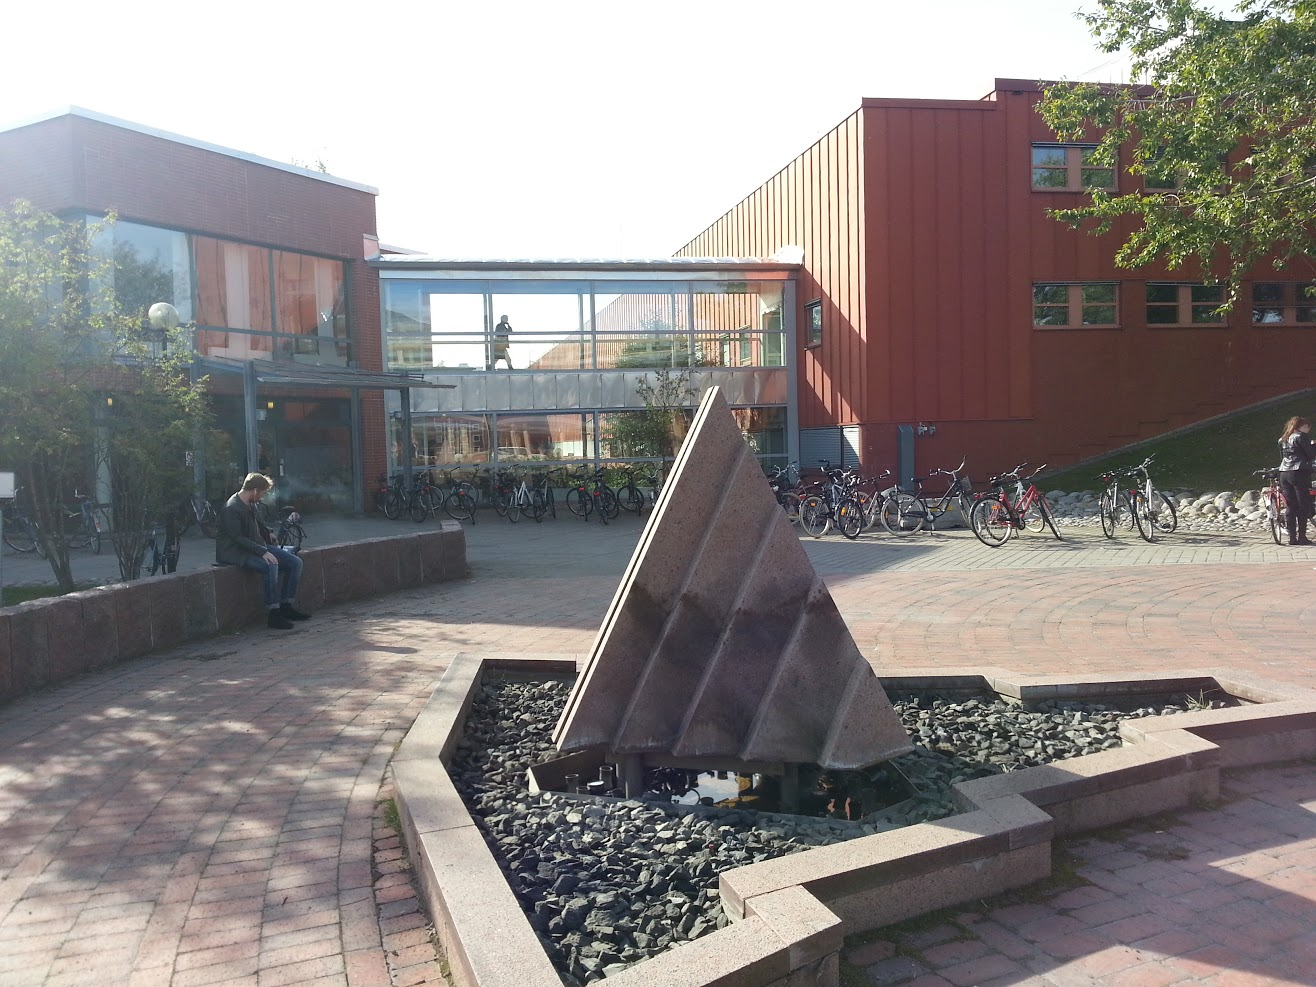
\includegraphics[width=0.32\textwidth]{media/campus_lulea.jpg}
	\par\textit{Lulea's University Campus}
\end{center}


%12345678901234567890123456789012345678901234567890123456789012345678901234567890
Eventually, the third semester of our master program came to an end. 
As a next step, we had to do our thesis in the partner host we have selected. 
At this point, we took separate ways with my fellow {\sc perccom} friends 
until we meet again in France for presenting our thesis work. 




%-----------------------------------------------------------
\NewsItem{A never ending journey}

%12345678901234567890123456789012345678901234567890123456789012345678901234567890
The {\sc perccom} master experience was unique and life changing for me. 
I meet so many different people from various cultures and backgrounds. 
Even so we were very different we end up being close, reliable, and great friends.
Strong bonds are connecting our cohort, we still keep contact with most of the 
fellow participants, we talk over skype, we update our contact and address details 
on a shared document, we send post cards during Easter, Christmas, 
or on New Years Eve.
All those magical moments I spend during my master in all these different countries 
are carved deeply in my memories and thoughts. 
The story does not ends here, we are organising meetings with my {\sc perccom} 
fellows at least once a year in various countries. 
From time to time we even spend holidays together, like spending New Years Eve on 
Alps. 
However, I wish I could turn back time and relive this enjoyable and 
unique journey over again. 


%12345678901234567890123456789012345678901234567890123456789012345678901234567890
As a conclusion, I would like to urge young students, still under-graduated, to 
follow my path and not to focus only on mainstream choice for their post-graduate 
degree. 
Getting a degree from a highly ranked University is of paramount importance. 
However, stressing mentally and over-pushing yourself to its limits very time 
it is not healthy. 
Many opportunities are available with various scholarships that European Union 
offers to study, travelling, do something different, get experience, and make 
new friends.
\textit{Also, we should all keep in mind that nobody will remember the time spend on studying 
or working, but instead all the crazy moments with joy and fun we had with friends.}

 
 
%---------------------------------------------------------------------------------------- 
\NewsItem{Acknowledgements}

%12345678901234567890123456789012345678901234567890123456789012345678901234567890
I would like to  thank, first of all, our {\sc perccom} Professors who wrote the 
proposals and got funds to create this project. 
Secondly, I like to thank the Erasmus Mundus Association for the funds and unique 
opportunity it gave us to travel and experience so many things in such a short 
period of time. 
Also, I would like to thank all my {\sc perccom} fellows and all the people I met 
abroad for their help, support, 
good time, and the unforgettable moments we lived together. 
Last but not least, I thank my parents for their support and motivation to take the 
risk to do something different. 
In addition, they urged me not to study all the time but instead to travel more 
around and get life experience on different fields.

\end{multicols}


\begin{center}
	\vspace{10pt}
	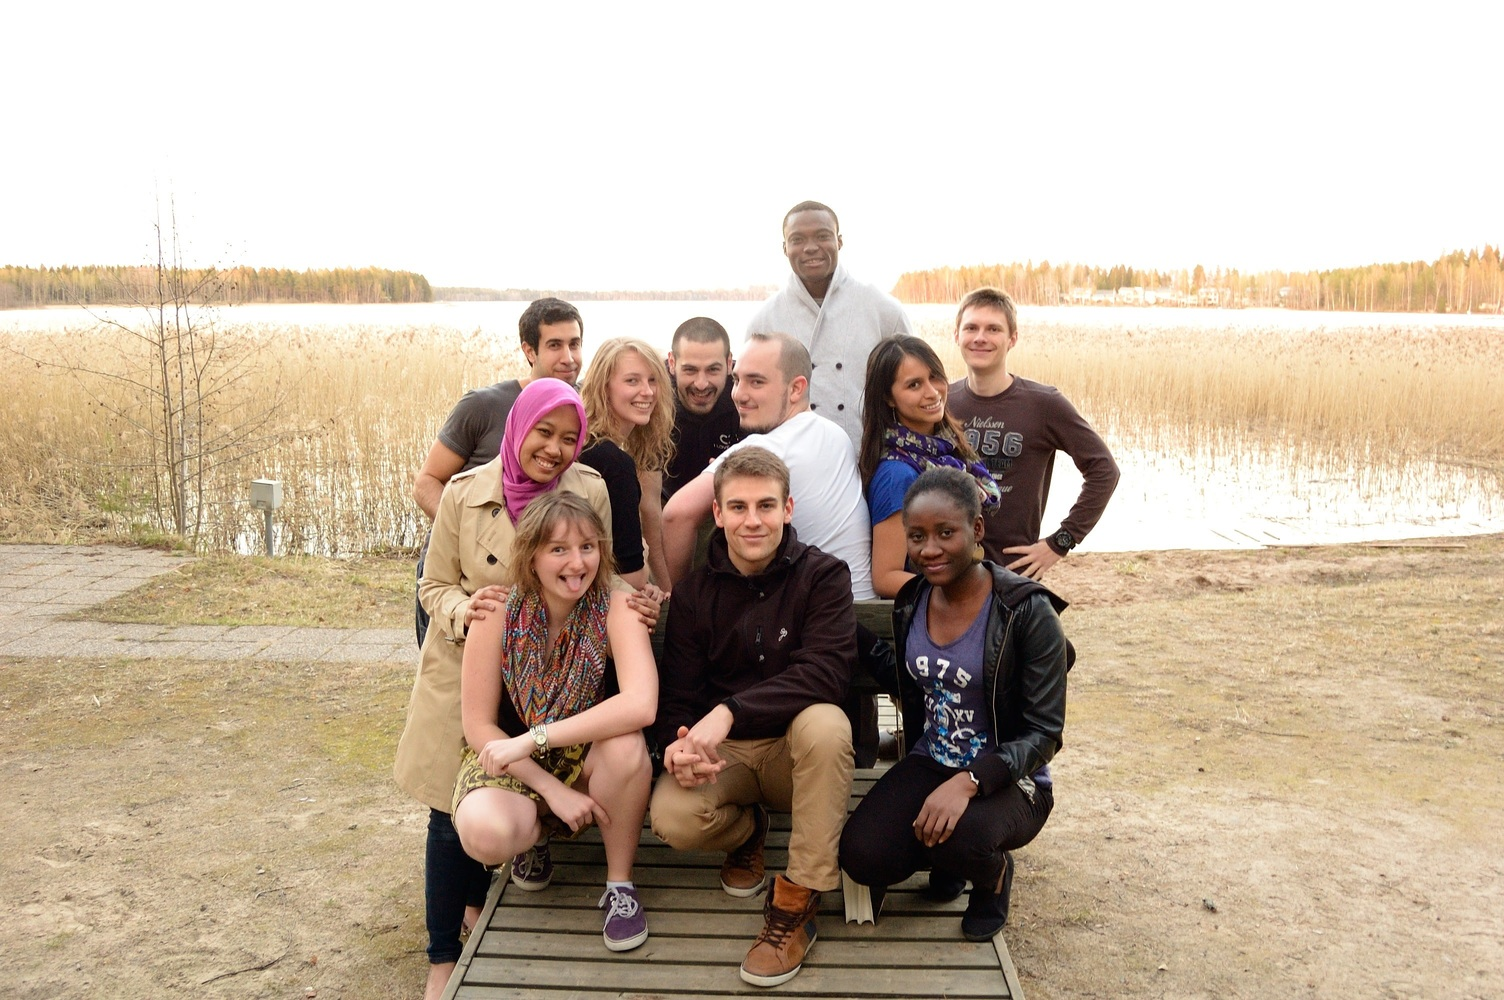
\includegraphics[width=1\linewidth]{media/perccom_family.jpg} % Example of an image taking up the total width of the page
	\vspace{10pt}
		\par\textit{Front row: Dorine, Baptiste, Zaine, Mid row: Alifia, Maike, Alexandre, Viki, Back row: Stefanos, Vlad, Fisayo, Vitalii}
\end{center}
%----------------------------------------------------------------------------------------



\end{document} 
